%
% rueckprojecktion.tex
%
% (c) 2023 Prof Dr Andreas Müller
%
\begin{figure}
\centering
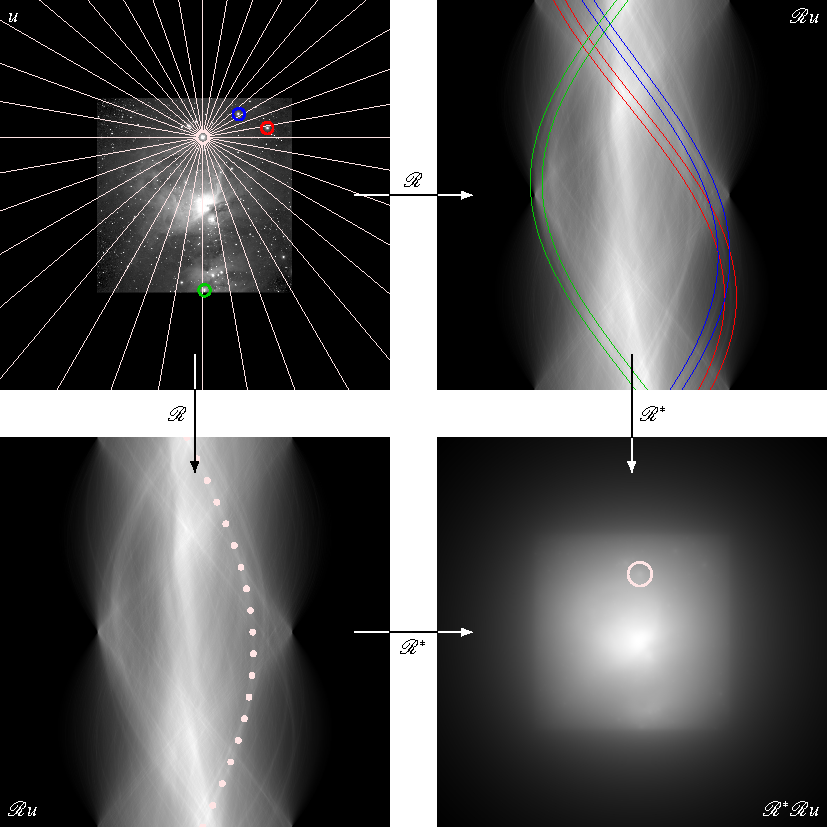
\includegraphics[width=\textwidth]{chapters/050-radon/images/rueckprojektion.pdf}
\caption{Die Rückprojektion $\mathscr{R}^*$ ist eine erste Approximation
der Inversen der Radon-Transformation.
In der Radontransformation werden helle Punkte des Bildes zu hellen
sinusähnlichen Kurven (farbig hervorgehobene Kurven in der Radon-Transformation
oben rechts).
Die Punkte einer solchen Kurve stehen für ein Integral über eine
Gerade, die durch den hellen Punkt gehen.
Summiert man diese Punkte (hellrote Punkte in der Radon-Transformation
unten rechts), entsteht ein höherer Wert als entlang einer weniger hellen
Kurve.
Überlagert sind aber auch Anteile von anderen Bildteilen, so entsteht
ein verschwommenes Bild, die Rückprojektion $\mathscr{R}^*u$.
\label{buch:radon:rueckprojektion:fig:rueckprojektion}}
\end{figure}
